\section{Application Demo Evidence}

\subsection{Demo environment and execution method}

All demonstrations used the real server and client implementations on
Windows. The server listened on TCP port 2121, while PASV or PORT dynamically
prepared UDP endpoints for data operations. The evidence process started the
server separately, connected real socket clients, executed public client
operations, recorded replies and comparisons, and removed all generated
files. A deterministic 16,384-byte binary payload and a two-line ASCII file
were used. No networking operation was mocked. Only the loss event was
controlled so the same retransmission could be reproduced.

\subsection{Overall results}

\begin{tabularx}{\textwidth}{l c X}
\toprule
Layer & Result & Coverage\\
\midrule
Core/unit & \pass\ 16/16 & Packet, CRC, GBN, ACK, loss, window, RTO, commands, paths\\
End-to-end & \pass\ 1/1 & Real server/client, PASV/PORT, ABOR, loss, 3 clients\\
Total & \pass\ 17/17 & Component and complete workflows\\
Compile/cleanup & \pass & Modules compile; data directories cleaned\\
\bottomrule
\end{tabularx}

\subsection{Demo A: Control channel and authentication}

\textbf{Objective.} Verify the TCP control connection, stateful login, and
standard reply codes.

\textbf{Execution.} One client connected and issued USER, PASS, NOOP, PWD,
HELP RETR, and QUIT over the same TCP socket.

\textbf{Result.} Replies 220, 331, 230, 200, 257, 214, and 221 were observed
in the expected order; login passed and the password was masked.

\begin{figure}[H]
\centering
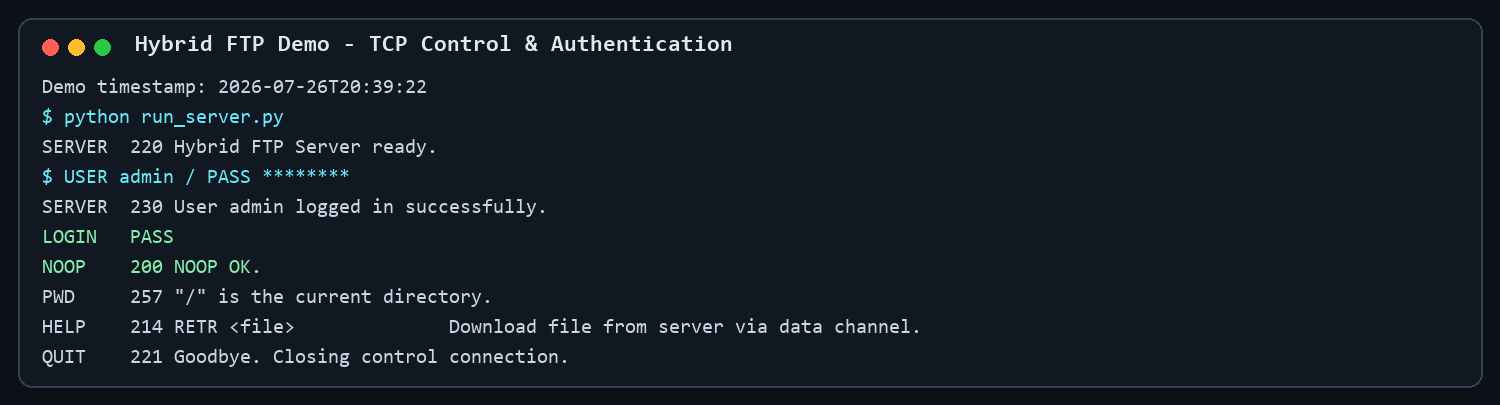
\includegraphics[width=\textwidth]{images/01-control-auth.png}
\caption{Actual control-channel authentication and session log.}
\end{figure}

\subsection{Demo B: Directory navigation}

\textbf{Objective.} Verify directory management inside the server sandbox.

\textbf{Execution.} The client executed MKD, UDP LIST, CWD, PWD, CDUP, and
RMD on \code{demo-folder}.

\textbf{Result.} Creation returned 257, the folder appeared in LIST, the
session path changed correctly, and removal returned 250. All steps passed.

\begin{figure}[H]
\centering
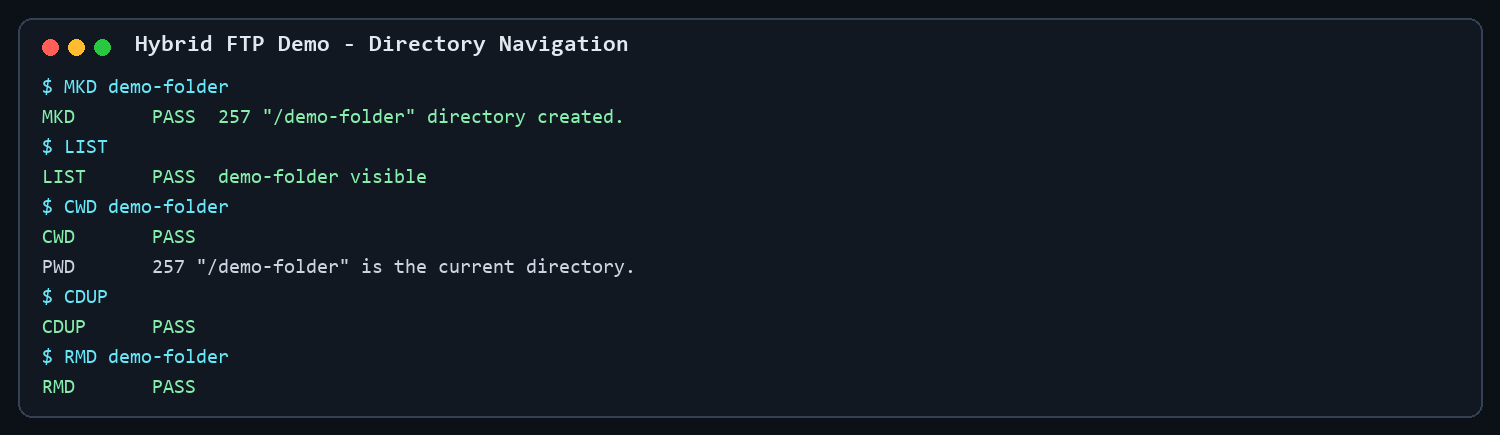
\includegraphics[width=\textwidth]{images/02-directory-navigation.png}
\caption{MKD, LIST, CWD, PWD, CDUP, and RMD evidence.}
\end{figure}

\subsection{Demo C: PASV transfer integrity}

\textbf{Objective.} Verify passive binary upload/download, metadata, and
end-to-end SHA-256.

\textbf{Execution.} Under TYPE I and PASV, the client uploaded and downloaded
a 16,384-byte file, compared its bytes, and requested SIZE, MDTM, STAT and
HASH SHA256.

\textbf{Result.} Both transfers passed, SIZE returned 16,384, metadata replies
were valid, and the local/server SHA-256 values matched.

\begin{figure}[H]
\centering
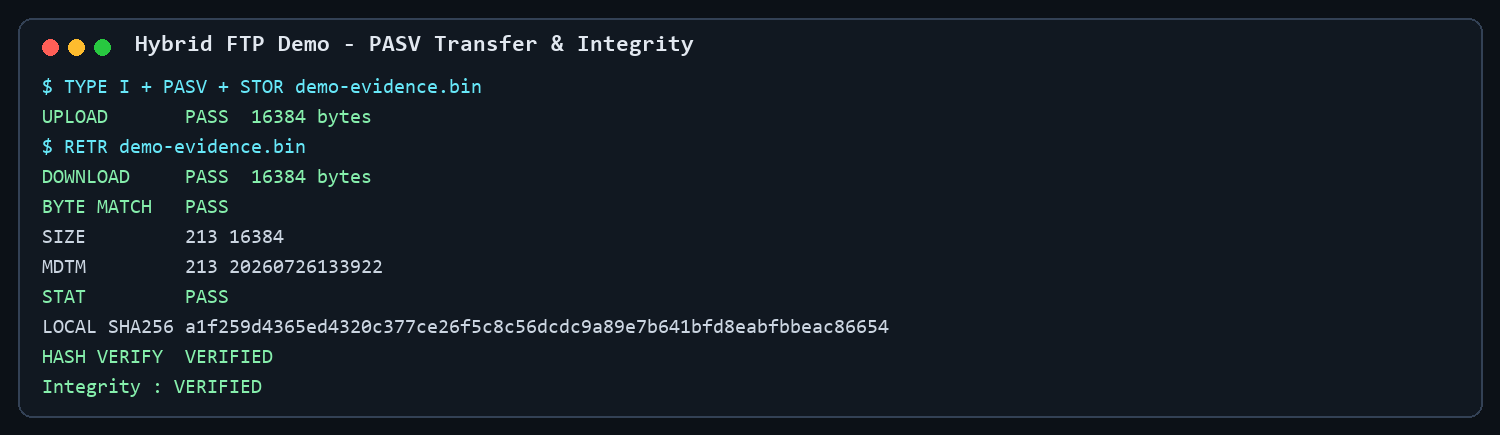
\includegraphics[width=\textwidth]{images/03-pasv-transfer-integrity.png}
\caption{PASV upload/download, metadata, and SHA-256 comparison.}
\end{figure}

\subsection{Demo D: ASCII and compressed representations}

\textbf{Objective.} Verify TYPE A canonicalisation and MODE C compression.

\textbf{Execution.} A two-line text file completed an ASCII round trip. The
binary payload then completed an upload/download under zlib compressed mode.

\textbf{Result.} ASCII upload, download, and newline comparison passed. The
decompressed binary output matched the original.

\begin{figure}[H]
\centering
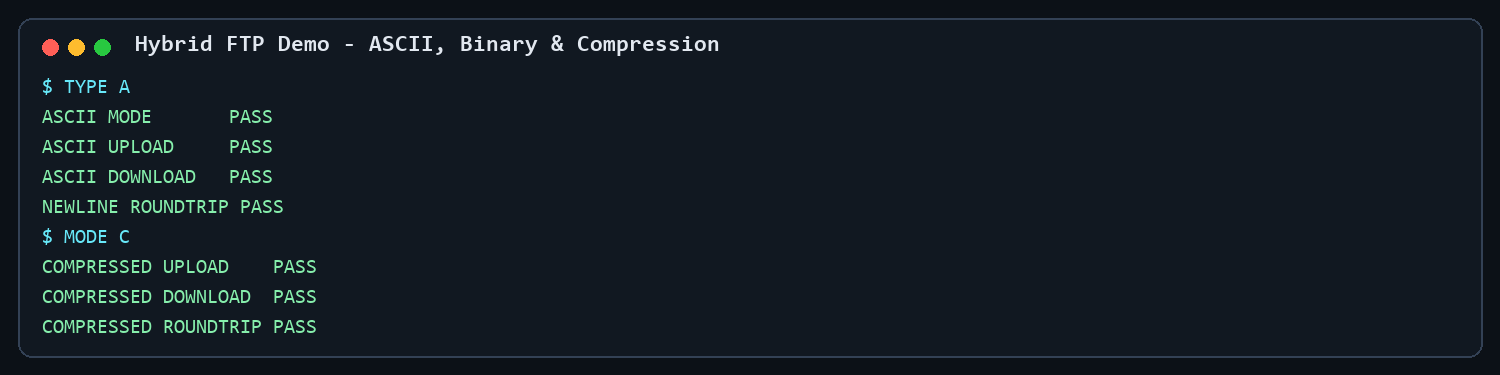
\includegraphics[width=\textwidth]{images/04-ascii-compression.png}
\caption{TYPE A newline round trip and MODE C compression.}
\end{figure}

\subsection{Demo E: Active PORT mode}

\textbf{Objective.} Verify runtime switching to the active data mechanism.

\textbf{Execution.} The client advertised its UDP endpoint with PORT. It then
uploaded, downloaded, byte-compared, and SHA-256-verified a binary file.

\textbf{Result.} PORT returned 200; both transfers and the byte comparison
passed; SHA-256 was verified.

\begin{figure}[H]
\centering
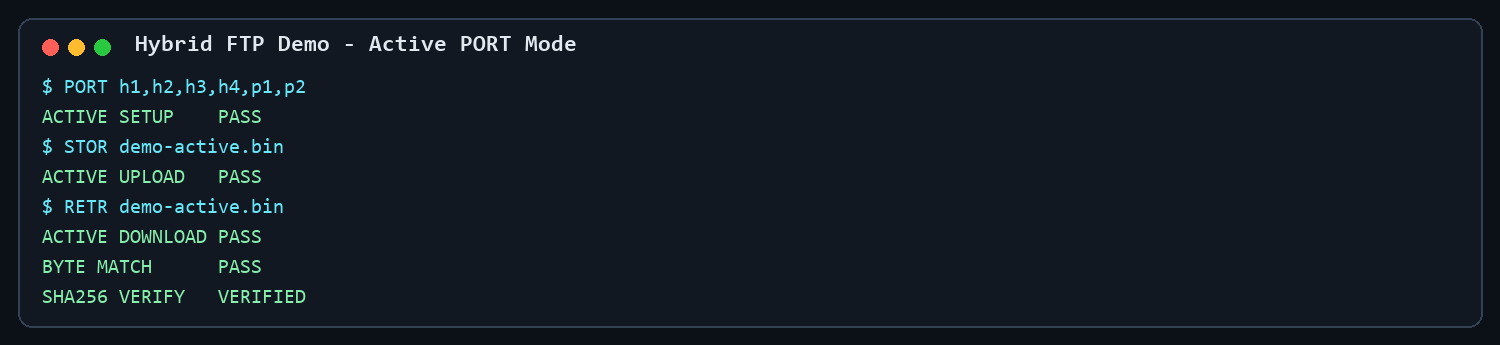
\includegraphics[width=\textwidth]{images/05-active-port.png}
\caption{Active-mode upload/download with byte and SHA-256 verification.}
\end{figure}

\subsection{Demo F: Extended file operations}

\textbf{Objective.} Verify rename, append, unique store, listing and deletion.

\textbf{Execution.} A 40-byte file was stored, renamed with RNFR/RNTO,
appended, measured, followed by STOU, NLST and deletion.

\textbf{Result.} SIZE became 80 bytes after append. The server generated a
unique filename; listing and both deletions passed.

\begin{figure}[H]
\centering
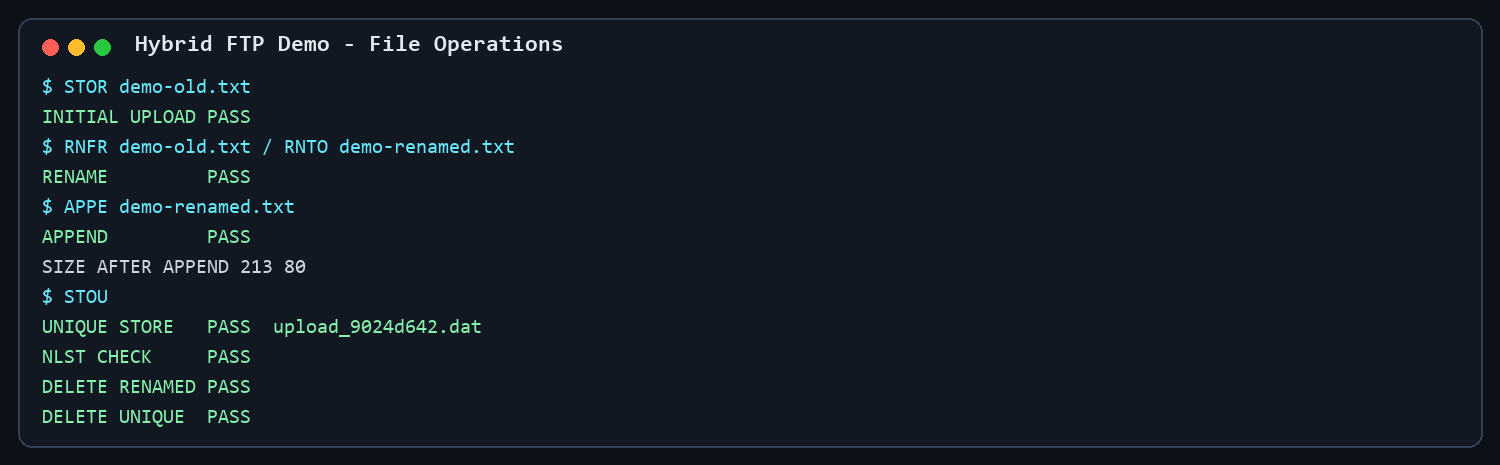
\includegraphics[width=\textwidth]{images/06-file-operations.png}
\caption{Rename, append, unique-store, listing, size, and deletion evidence.}
\end{figure}

\subsection{Demo G: Go-Back-N loss recovery}

\textbf{Objective.} Demonstrate recovery from a real missing DATA datagram.

\textbf{Execution.} A 20\% loss simulator deterministically dropped sequence
zero. The remaining sender, receiver, timer, ACK and UDP behaviour was real.

\textbf{Result.} The sender timed out at base zero, retransmitted the
outstanding flight, completed with one retransmission, and produced a
verified SHA-256 digest.

\begin{figure}[H]
\centering
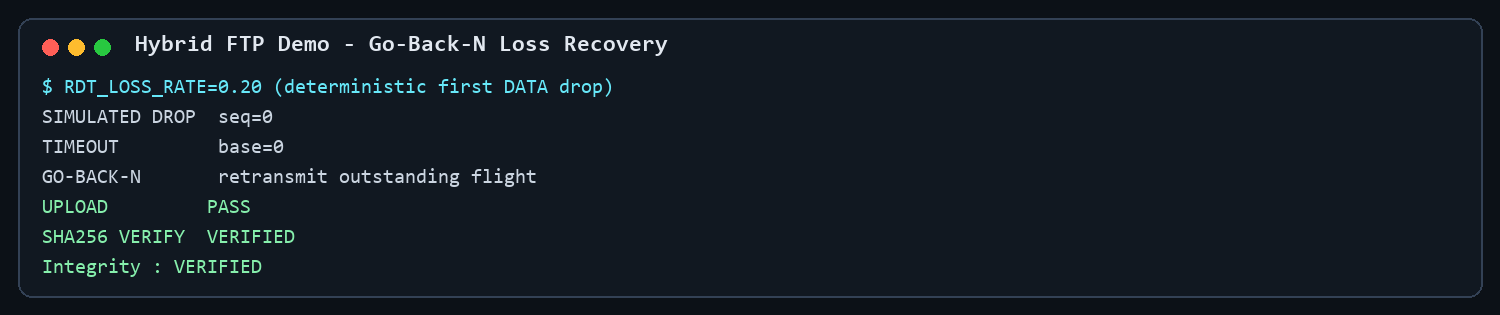
\includegraphics[width=\textwidth]{images/07-loss-recovery.png}
\caption{Deterministic DATA loss, timeout, retransmission, and verified hash.}
\end{figure}

\subsection{Demo H: Concurrent isolated sessions}

\textbf{Objective.} Verify multi-threaded session isolation.

\textbf{Execution.} Three independent clients concurrently logged in, opened
PASV endpoints, uploaded unique files, verified hashes, deleted the files,
and quit.

\textbf{Result.} All three clients passed login, upload, and SHA-256
verification. No worker timed out or produced a mismatched digest.

\begin{figure}[H]
\centering
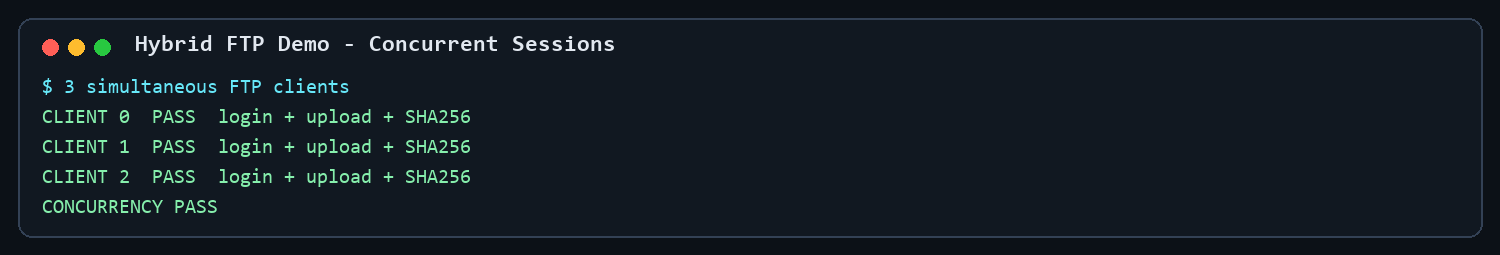
\includegraphics[width=\textwidth]{images/08-concurrency.png}
\caption{Three simultaneous authenticated client sessions.}
\end{figure}

\subsection{Evidence and test relationship}

\begin{lstlisting}
python -m unittest tests.test_core -v
python -m unittest tests.test_integration -v
python -m unittest discover -s tests -v
python tools/generate_demo_evidence.py
\end{lstlisting}

The E2E suite covers real TCP authentication, PASV/PORT UDP transfers,
binary SHA-256 verification, ASCII and compressed round trips, metadata,
STOU/APPE/rename, live ABOR, deterministic packet loss and retransmission,
three concurrent authenticated clients, and cleanup.

\begin{table}[H]
\centering
\begin{tabular}{lll}
\toprule
Demo & Requirement & Result\\
\midrule
A & TCP control and authentication & PASS\\
B & Directory management & PASS\\
C & PASV binary and SHA-256 & PASS / VERIFIED\\
D & ASCII and compression & PASS\\
E & Active PORT mode & PASS / VERIFIED\\
F & Extended file operations & PASS\\
G & Go-Back-N loss recovery & PASS / VERIFIED\\
H & Three concurrent clients & PASS\\
\bottomrule
\end{tabular}
\caption{Summary of observed demonstration results.}
\end{table}